\section{Explaining Type Errors With Traces}
\label{sec:interactive}

A trace, on its own, is too detailed to be
a good explanation of the type error. One approach
is to use the witness input to step through the
program with a \emph{debugger} to observe how
the program evolves.
%
This route is problematic for two reasons.
%
First, existing debuggers and interpreters for
typed languages (\eg\ \ocaml) typically require
a type-correct program as input.
%
Second, we wish to have a quicker way to get
to the essence of the error, \eg\ by skipping
over irrelevant sub-computations, and focusing
on the important ones.

Next, we present a novel way to debug executions.
%
First, we develop a notion of a \emph{reduction graphs}
and extend our semantics with a form of \emph{tracing}
so that they incrementally collect the edges
in the graph (\S~\ref{sec:inter-semant}).
%
Next, we express a set of common \emph{interactive debugging}
steps as graph traversals (\S~\ref{sec:traversing-graph}), yielding
an novel interactive debugger that allows the user
to effectively visualize \emph{how} the program goes (wrong.)

\subsection{Tracing Semantics}
\label{sec:inter-semant}
%
\begin{figure*}[t]
\relDescription{Computing Sub-Terms}
\begin{gather*}
\begin{array}{lcl}
\subtermssym                 & \dcolon & e \to \tr \\
\subterms{\eapp{e_1}{e_2}}   & \defeq & \subterm{\eapp{e_1}{e_2}}{e_1}; \subterm{\eapp{e_1}{e_2}}{e_2} \\
\subterms{\eplus{e_1}{e_2}}   & \defeq & \subterm{\eplus{e_1}{e_2}}{e_1}; \subterm{\eplus{e_1}{e_2}}{e_2} \\
\subterms{\eif{e_1}{e_2}{e_3}}   & \defeq & \subterm{\eif{e_1}{e_2}{e_3}}{e_1}; \\
                                &        & \subterm{\eif{e_1}{e_2}{e_3}}{e_2}; \\
                                &        & \subterm{\eif{e_1}{e_2}{e_3}}{e_3} \\
\subterms{\elet{x}{e_1}{e_2}}   & \defeq & \subterm{\elet{x}{e_1}{e_2}}{e_1}; \\
                                &        & \subterm{\elet{x}{e_1}{e_2}}{e_2} \\
\subterms{\efun{x}{e}}       & \defeq & \subterm{\efun{x}{e}}{e} \\
\subterms{e}                 & \defeq & \bullet
\end{array}
\end{gather*}
\judgementHead{Traced Evaluation}{\stepg{e}{\su}{\tr}{e}{\su}{\tr}}
\begin{gather*}
\inference[\recontext]
  {\stepg{e}{\su}{\tr}{e_1}{\su_1}{\tr_1}}
  {\stepg{C[e]}{\su}{\tr}{C[e_1]}{\su_1}{\singlestep{C[e]}{C[e_1]}; \subterms{C[e_1]}; \tr_1}}
\\ \\
\inference[\reappgood]
  {\pair{\efun{x}{e}}{\su_2} = \force{v_1}{\tfun{\thole{}}{\thole{}}}{\su_1}}
  {\stepg{\eapp{v_1}{v_2}}{\su_1}{\tr}
         {e\sub{x}{v_2}}{\su_1;\su_2}{\singlestep{\eapp{v_1}{v_2}}{e\sub{x}{v_2}}; \subterms{e\sub{x}{v_2}}; \tr}}
\\ \\
\inference[\reappbad]
  {\pair{\stuck}{\su_2} = \force{v_1}{\tfun{\thole{}}{\thole{}}}{\su_1}}
  {\stepg{\eapp{v_1}{v_2}}{\su_1}{\tr}{\stuck}{\su_1;\su_2}{\singlestep{\eapp{v_1}{v_2}}{\stuck}; \tr}}
\end{gather*}
\caption{A selection of the operational semantics from
  Figure~\ref{fig:operational}, extended to collect a full reduction
  graph.}
\label{fig:interactive}
\end{figure*}

\paragraph{Reduction Graphs}
%
A \emph{steps-to} edge is a pair of expressions \singlestep{e_1}{e_2}, which
intuitively indicates that $e_1$ steps, in a single step, to $e_2$.
%
A \emph{sub-term} edge is a pair of expressions \subterm{e_1}{e_2}, which
intuitively indicates that $e_1$ contains $e_2$ as a sub-expression.
%
A \emph{reduction graph} is a set of edges:
$$\tr ::= \bullet \spmid \singlestep{e}{e}; \tr \spmid \subterm{e}{e}; \tr$$

\paragraph{Tracing Semantics}
%
We extend the transition relation (\S~\ref{sec:semantics}) to
collect the set of edges corresponding to the reduction graph.
%
Concretely, we extend the operational semantics to
a relation of the form $\stepg{e}{\vsu}{\tr}{e'}{\vsu'}{\tr'}$
where $\tr'$ collects the edges of the transition.

\paragraph{Collecting Edges}
%
Next, we describe the general recipe for extending a transition
rule to collect edges, and provide a selection of examples
in Figure~\ref{fig:interactive}.
%
The steps-to edges are collected by recording the consequent of
each original rule in the trace. That is, each original judgment
\step{e}{\vsu}{e'}{\vsu'} becomes
\stepg{e}{\vsu}{\tr}{e'}{\vsu'}{\singlestep{e}{e'}; \tr}.
%
The sub-term edges are delegated to a helper function \subtermssym\
which adds edges from an expression to each of its
\emph{immediate} sub-expressions.
%
We collect \subtermssym edges after each transition,
to get the following template for the small-step relation:
\[
\stepg{e}{\vsu}{\tr}{e'}{\vsu'}{\singlestep{e}{e'}; \subterms{e'}; \tr}
\]


\subsection{Interactive Debugging}
\label{sec:traversing-graph}

Next, we show how to build a visual interactive debugger
from the traced semantics, by describing the visualization
\emph{state} \ie\ what the user sees at any given moment,
the set of \emph{commands} available to user and what
they do, and finally how we use a command to \emph{update}
the visualization state. In the sequel, for clarity of
exposition, we assume we have a (global) trace:
$\stepg{e_0}{\emptysu}{\bullet}{e_n}{\_}{\tr}$, where
$e_0$ and $e_n$ are the \emph{initial} and \emph{final}
expressions respectively.

\paragraph{Visualization State}
%
A \emph{visualization state} @VState@ is a \emph{directed graph}
whose vertices are expressions and whose edges are such
that each vertex has at most one predecessor and at most one
successor. In other words, the visualization state looks
like a set of linear lists of expressions as shown in Figure~\ref{fig:nanomaly-factorial}.
%
The \emph{initial state} is the graph containing a single
edge linking the initial and final expressions.

\paragraph{Commands}
Our debugger supports the following \emph{commands}, each of which
is parameterized by a single expression (vertex) selected from the
(current) visualization state:
%
\begin{itemize}
%
\item \stepforwardsym, \stepbackwardsym:
      show result of a single step forward or backward respectively,
%
\item \jumpforwardsym:
      show result of taking multiple steps (a \emph{``big''} step)
      upto the first beta-reduction forward or backward respectively,
%
\item \stepintosym:
      show result of stepping into a function call in a sub-term,
      isolating it from the context,

\item \stepoversym:
      show result of skipping over a function call in a sub-term.
\end{itemize}

%\begin{figure}[t]
\centering
% \begin{minipage}{0.49\linewidth}
\begin{mcode}
(*\putBefore*) :: (*\vstate*) -> (*\expr*) -> (*\expr*) -> (*\vstate*)
(*\putAfter*)  :: (*\vstate*) -> (*\expr*) -> (*\expr*) -> (*\vstate*)
(*\putRoot*)   :: (*\vstate*) -> (*\expr*) -> (*\vstate*)
(*\getRoot*)   :: (*\vstate*) -> (*\expr*) -> (*\expr*)
(*\getPath*)      :: (*\tr*) -> (*\expr*) -> [(*\expr*)]

(*\getSubterms*) :: (*\vstate*) -> (*\expr*) -> [((*\expr*),(*\ctx*))]
(*\applyCtx*)    :: (*\vstate*) -> (*\expr*) -> (*\ctx*) -> (*\expr*)

findApp    :: (*\vstate*) -> (*\expr*) -> Maybe ((*\expr*),(*\ctx*))
findValue  :: (*\vstate*) -> (*\expr*) -> (*\expr*)

data (*\cmd*) = (*\stepforwardc*) | (*\stepbackwardc*)
         | (*\jumpforwardc*) | (*\jumpbackwardc*)
         | (*\stepoverc*)    | (*\stepintoc*)
\end{mcode}
% data (*\ctx*)
\caption{Graph manipulation and traversal API.}
\label{fig:graph-api}
\end{figure}
% \end{minipage}
% \begin{minipage}{0.49\linewidth}
\begin{figure}[t]
\begin{mcode}
(*\findExpr*) :: (*\vstate*) -> (*\cmd*) -> (*\expr*) -> Maybe (*\expr*)
(*\findExpr*) v c e = case c of
  (*\stepforwardc*) -> 
    let p = (*\getPath*) v e in (p!!1)
  (*\stepbackwardc*) -> 
    let p = (*\getPath*) v ((*\getRoot*) v e) in last p
  (*\jumpforwardc*) -> case (*\findExpr*) v (*\stepforwardc*) e of
    $\eapp{v_1}{v_2}$ -> Just ($\eapp{v_1}{v_2}$)
    e'   -> (*\findExpr*) v c e'
  (*\jumpbackwardc*) -> case (*\findExpr*) v (*\stepbackwardc*) e of
    $\eapp{v_1}{v_2}$ -> Just ($\eapp{v_1}{v_2}$)
    e'   -> (*\findExpr*) v c e'
  (*\stepintoc*) -> findApp v e
  (*\stepoverc*) -> case findApp v e of
    Nothing       -> Nothing
    Just (e', cx) -> applyCtx v (crunch v e') cx

(*\updState*) :: (*\vstate*) -> (*\cmd*) -> (*\expr*) -> Maybe (*\vstate*)
(*\updState*) v c e = case (*\findExpr*) v c e of
  Nothing -> Nothing
  Just e' -> Just (*\$*) case c of
    (*\stepforwardc*) -> (*\putAfter\ v e e'*)
    (*\stepbackwardc*)    -> (*\putBefore\ v e e'*)
    (*\jumpforwardc*) -> (*\putAfter\ v e e'*)
    (*\jumpbackwardc*)    -> (*\putBefore\ v e e'*)
    (*\stepintoc*)    -> (*\putRoot\ v e' (crunch v e') *)
    (*\stepoverc*)    -> (*\putAfter\ v e e'*)
\end{mcode}
% \end{minipage}
% \[
% \begin{array}{lcl}
% \stepforward{G}{p}{e_i}  &\defeq& \left\{\begin{array}{ll}
%     e_j, & \text{where } \singlestep{e_i}{e_j} \in G
%                          \end{array}\right\} \\ \\
% \stepbackward{G}{p}{e_i}  &\defeq& \left\{\begin{array}{ll}
%     e_j, & \text{where } \singlestep{e_j}{e_i} \in G \text{ and } e_j \in p
%                          \end{array}\right\} \\ \\
% \jumpforward{G}{p}{e_i} &\defeq& \text{let } e_j = \stepforward{G}{p}{e_i} \text{ in }
%                          \left\{\begin{array}{ll}
%                          e_j, & \text{if } e_j = \eapp{v_1}{v_2} \\
%                          \jumpforward{G}{p}{e_{j}}, & \text{otherwise}
%                          \end{array}\right\} \\ \\
% \jumpbackward{G}{p}{e_i} &\defeq& \text{let } e_j = \stepbackward{G}{p}{e_i} \text{ in }
%                          \left\{\begin{array}{ll}
%                          e_j, & \text{if } e_j = \eapp{v_1}{v_2} \\
%                          \jumpbackward{G}{p}{e_{j}}, & \text{otherwise}
%                          \end{array}\right\} \\ \\
% \stepinto{G}{p}{e_i} &\defeq& \left\{\begin{array}{ll}
%                          e\sub{x}{v_2}, & \text{if } e_i = C[\eapp{v_1}{v_2}] \text{ and } \singlestep{\eapp{v_1}{v_2}}{e\sub{x}{v_2}}
%                          \end{array}\right\} \\ \\
% \stepover{G}{p}{e_i} &\defeq& \left\{\begin{array}{ll}
%                          C[v], & \text{if } e_i = C[\eapp{v_1}{v_2}] \text{ and } \multistep{\eapp{v_1}{v_2}}{v}
%                          \end{array}\right\}
% \end{array}
% \]
\caption{Rules for updating the reduction graph given a command and a selected expression. \texttt{updState} returns \texttt{Nothing} if the command was not applicable. % \stepintosym and \stepoversym require a traversal of the
  % sub-term edges to decompose $e_i$ into the target expression
  % \eapp{v_1}{v_2} and the context $C$.  \ES{these rules are quite ugly and waste space..}
}
\label{fig:traversing-graph}
\end{figure}

\begin{figure*}[t]
\[
\begin{array}{lcl}
\stepforward{G}{p}{e_i}  &\defeq& \begin{array}{ll}
    e_j, & \text{where } \singlestep{e_i}{e_j} \in G
                         \end{array}\right\} \\ \\
\stepbackward{G}{p}{e_i}  &\defeq& \left\{\begin{array}{ll}
    e_j, & \text{where } \singlestep{e_j}{e_i} \in G \text{ and } e_j \in p
                         \end{array}\right\} \\ \\
\jumpforward{G}{p}{e_i} &\defeq& \text{let } e_j = \stepforward{G}{p}{e_i} \text{ in }
                         \left\{\begin{array}{ll}
                         e_j, & \text{if } e_j = \eapp{v_1}{v_2} \\
                         \jumpforward{G}{p}{e_{j}}, & \text{otherwise}
                         \end{array}\right\} \\ \\
\jumpbackward{G}{p}{e_i} &\defeq& \text{let } e_j = \stepbackward{G}{p}{e_i} \text{ in }
                         \left\{\begin{array}{ll}
                         e_j, & \text{if } e_j = \eapp{v_1}{v_2} \\
                         \jumpbackward{G}{p}{e_{j}}, & \text{otherwise}
                         \end{array}\right\} \\ \\
\stepinto{G}{p}{e_i} &\defeq& \left\{\begin{array}{ll}
                         e\sub{x}{v_2}, & \text{if } e_i = C[\eapp{v_1}{v_2}] \text{ and } \singlestep{\eapp{v_1}{v_2}}{e\sub{x}{v_2}}
                         \end{array}\right\} \\ \\
\stepover{G}{p}{e_i} &\defeq& \left\{\begin{array}{ll}
                         C[v], & \text{if } e_i = C[\eapp{v_1}{v_2}] \text{ and } \multistep{\eapp{v_1}{v_2}}{v}
                         \end{array}\right\}
\end{array}
\]
\caption{Rules for updating the reduction graph given a command and a selected expression. \texttt{updState} returns \texttt{Nothing} if the command was not applicable. % \stepintosym and \stepoversym require a traversal of the
  % sub-term edges to decompose $e_i$ into the target expression
  % \eapp{v_1}{v_2} and the context $C$.  \ES{these rules are quite ugly and waste space..}
}
\label{fig:traversing-graph}
\end{figure*}


\paragraph{Update}
Figure~\ref{fig:traversing-graph} shows how we update the state
for each command.
%
The procedure \findExpr{\vstate}{\cmd}{e} traverses $\tr$
and the current visualization state to compute the new
expression that should be added to the visualization state;
and \updState{\vstate}{\cmd}{e} then updates the graph
by inserting the new expression appropriately, using
one of the following graph manipulating functions:
%
\putBefore{\vstate}{e}{e'} (resp. \putAfter{\vstate}{e}{e'})
returns the modified version of \vstate\ where $e'$ is the
immediate predecessor of $e$ (resp.\ the immediate successor of $e$);
%
\putRoot{\vstate}{e}{e'} returns the modified version of \vstate
extended with a new root vertex $e$ with successor $e'$.
%
% @getRoot vs e@ returns the vertex (expression) obtained
% by transitively following the predecessors of @e@ until a
% source vertex.

@getNext vs e@ returns the immediate successor of @e@ in $\tr$.
%
@getPrev vs e@ computes the path @p@ between @e@ and its immediate
predecessor in the current visualization, and then returns @e@'s immediate
predecessor along @p@.
%
@getSubterms vs e@ traverses the sub-term edges to decompose an
expression into a list of sub-expressions paired with their context.
%
@applyCtx vs e ctx@ applies @ctx@ to @e@, traversing the sub-term edges
in reverse to find the super-term of @e@.
%
\hbox{@findApp vs e@} builds on top of @getSubterms@ to find the first
application sub-term (if any), \ie the first sub-term that looks like
$\eapp{v_1}{v_2}$.
%
@findVal vs e@ traverses the single-step edges to find the final value
that @e@ reduces to.
%
% Note that the sub-term edges $\searrow$ allow us to decompose an
% expression into a sub-expression and the surrounding context, thus
% enabling the \stepintosym\ and \stepoversym\ traversals.

% \RJ{EXAMPLE of interaction from overview goes here}
\begin{figure}[t]
\centering
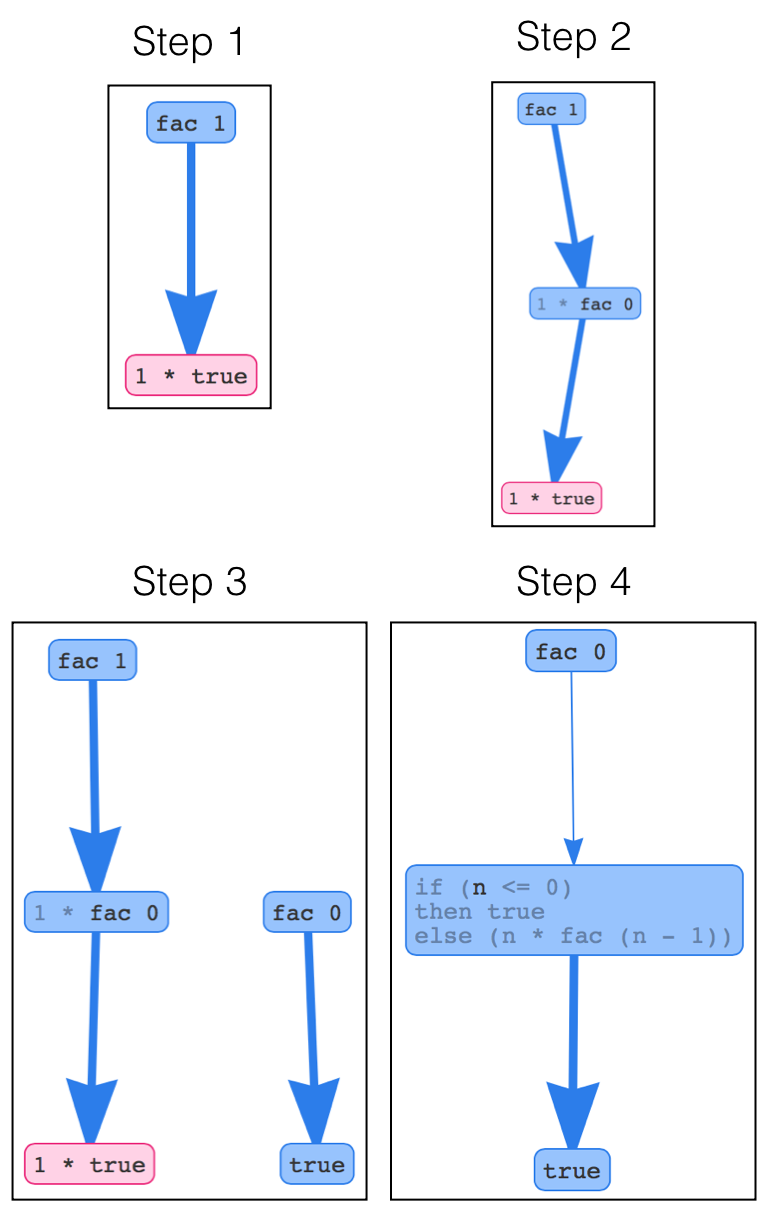
\includegraphics[width=0.8\linewidth]{fac-steps.png}
\caption{A sequence of interactions with the trace of
  \texttt{fac 1}. The stuck term is red, in each node the redex is
  highlighted. Thick arrows denote a multi-step transition, thin arrows
  denote a single-step transition. We start in step 1. In step 2 we jump
  forward from the witness to the next function call. In step 3 we step
  into the recursive \texttt{fac 0} call, which spawns a new ``thread''
  of execution. In step 4 we take a single step forward from
  \texttt{fac 0}.} % (hiding the context for space).}
\label{fig:nanomaly-factorial}
\end{figure}

%
%
%The initial path $p$ is required for the backward-steps as a node may
%have multiple incoming $\leadsto$ edges, \eg
%\singlestep{\eplus{1}{2}}{3} and \singlestep{\eplus{2}{1}}{3}.
%
